\section{Evaluation}

The proposed design has been simulated by ISim for implementation on Xilinx Sparttan6 XC6SLX4 hardware platform, where 32MB on-chip memory is used. 
The data path is simulated by using Verilog and Python script. 
The test bench is generated through Python and it send to ISim simulator. 
The instruction for insert/delete is executed based on the 1 bit opcode value. 
Internal logic of FPGA determines the replacement operation based on two consecutive opcode. 
Unless otherwise stated, a random sequence of insert/delete operations is used.

\subsection{Sensitivity Analysis}

We explore how the results (frequency, execution time and throughput) change with the number of levels.
The execution time per level is calculated as:
\begin{eqnarray}
t &=&  \frac{3}{f}
\end{eqnarray}
where $f$ is the frequency. 
Throughput ($\tau$) is calculated as:
\begin{eqnarray}
\tau &=&  \frac{\omega \times  f}{\chi}
\end{eqnarray}
 where $\omega$ is the bit length, $f$ is the clock frequency and $\chi$ is the number of clock cycles required to compute one {\it insert-delete} operation.
We use the number of levels ($\beta$) and bit length ($\omega$) interchangeably. 
The number of elements in the heap is $2^\omega-1 = 2^\beta -1$. 

 \begin{table}
 \begin{center}
 \caption{Variation of frequency, execution time and throughput with the number of levels.}
\label{table1}
\begin{tabular}{ |c|c|c|c| }
 \hline
 Number of & Frequency ($f$) & Execution Time& Throughput ($\tau$) \\
 Levels ($\beta$) & (MHz)& (ns)& (GB/Sec)\\
 \hline
 \hline
 4 & 318.8 & 9.41 & 1.27\\
 8 & 232.8 & 12.88 & 1.85\\
 10 & 212 & 14.15 & 2.12 \\
 12 & 210 & 14.25 & 2.52 \\
 16 & 207.2 & 14.5 & 3.31\\
 20 & 173.4 & 17.3 & 3.46 \\
 24 & 171.6 & 17.48 & 4.10\\
 \hline
\end{tabular}
\end{center}
\end{table}

From Table \ref{table1}, we found that the obtained clock frequency is not constant, it is inversely proportion to the bit length ($\beta$). 
We obtain maximum frequency = 318.8 MHz for $\beta = 4$, and minimum frequency 171.6 MHz $\beta = 24$. 
Execution time is directly proportion to frequency and inversely proportion to $\beta$ because it takes 3 cycles (worst case) per stage to complete the task. 
Increasing the number of levels, both clock frequency and execution time increase, but the throughput also increases.
As we have designed a fully pipelined architecture, the output can be obtained in each clock cycle as shown in Figure \ref{clock2}. 
For the rest of experiments, we use $\beta = 24$.

\subsection{Hardware Cost and Response Time}

The hole minimization technique reduces both hardware cost and response time.
The two optimization techniques further improve them.
The hardware sharing technique contributes to reducing the hardware cost, and the {\it replacement} operation shorten the response time further.

Table~\ref{table2} shows results of the hardware cost measurement.
Before applying the hole minimization technique, the number of comparators, filp-flops, LUTs and slices is 32, 1400, 3165, and 4870, respectively.
By applying the technique, it is reduced by 0.00\%, 42.14\%, 37.76\%, and 41.07\%, respectively.
The hardware sharing technique reduces it even further by 50.00\%, 3.70\%, 6.60\%, and 4.88\%, respectively.

\begin{table}
 \begin{center}
 \caption{Hardware cost results. LUT stands for look-up table.}
\label{table2}
\begin{tabular}{|c|c|c|c|c|}
 \hline
 Design  & Comparator  & Flip-flop & LUT &Slice \\
 \hline
 \hline
Without hole minimization & 32 & 1400 & 3165 & 4870 \\
 \hline
With hole minimization & 32 & 810 & 1970 & 2870 \\
  \hline
With hardware sharing & 16 & 780 & 1840 & 2730 \\
\hline
\end{tabular}
\end{center}
\end{table}

The hole minimization technique also improves the responsem time as shown in Table~\ref{table3}.
The hole minimization technique reduces the response time from 2010 to 1920, which corresponds to 4.48\% reduction.
By introducing the {\it replacement} operation, the response time is further reduced by 30.36\%.

\begin{table}
 \begin{center}
 \caption{Response time results.}
\label{table3}
\begin{tabular}{ |c|c|}
 \hline
 Design  &  Response Time (ms) \\
 \hline
Without hole minimization & 2010 \\
  \hline
With hole minimization & 1920 \\
  \hline
With replacement & 1337 \\
  \hline
\end{tabular}
\end{center}
\end{table}

The impact of the {\it replacement} operation is dependent on the sequence of operations.
Figure~\ref{random} compares the response time according to the sequence of operations.
When only {\it insert} operations come, there will be no hole created, which gives us second to the best response time.
The best case is when insert/delete operations come in an alternative fashion.
In this case, all pair of insert/delete operations can be replaced with the replacement operation.
The worst case is when only delete operations come right after only insert operations are processed.
In this case, none of operations can benefit from the replacement operations while many holes are created.
The response time of a random sequence is in-between the best and worst cases.

\begin{figure}[!ht]
  \centering
  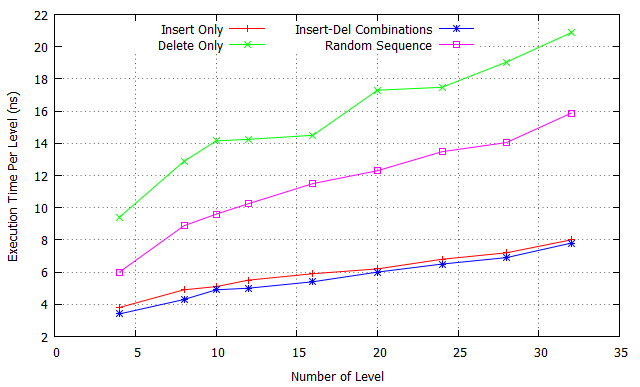
\includegraphics[width=8.0cm]{Figures/random.png}
      \caption{Execution time for different sequence of operations.}
    \label{random}
\end{figure}

\subsection{Comparison with Existing Techniques}

The three techniques proposed in this paper (hole minimization, hardware sharing, and replacement operation) offers more efficient implementation of a priority queue when compared with previous works.
Table~\ref{table4} compares the hardware cost and response time with existing techniques.
Since different designs address different issues and implemented in different platform, the comparison is made based on complexity analysis.

\begin{table*}
 \begin{center}
 \caption{Hardware cost and performance comparison with previous works. $n$ denotes the number of nodes.}
\label{table4}
\begin{tabular}{ |c|c|c|c|c|c|c|c|c| }
 \hline
 Design  & Comparator  & Flip-flop & SRAM & LUT &Max Frequency & Throughput ($\tau$) & Execution & Complete \\
  & ($\kappa$)& ($F$)& ($M$) &  & ($f$) (MHz) & (GB/Sec) & Time & Tree ?\\
 \hline
 \hline
 \cite{hw8} & $2^\beta$ & $2^{\beta +1}$& 0 & 8560 & - & - & $O(1)$ & Yes\\
 \hline
 \cite{hw11} & $2 \times \beta$ & $2^{\beta +1}$ & 0 & 1411 & - & - & $O(\log n)$ & Yes\\
 \hline
 \cite{fpga1} & $2 \times \beta$ & $2 \times \beta$ & $2 \times \beta$ & - & 180 &6.4 & $O(1)$ & No\\
 \hline
 \cite{hw2} & $2 \times \beta$ & $2 \times \beta$ & $2 \times \beta$ & - & 35.56 &10 & $O(1)$ & No\\
 \hline
{\bf Proposed} & {\bf $\frac{\beta}{2}$} & {\bf $\beta$} & {\bf $\beta$} & {\bf 1840} & {\bf 171.6} & {\bf 4.10} & {\bf $O(1)$} & {\bf Yes}\\
 \hline
\end{tabular}
\end{center}
\end{table*}

When compared to reference~\cite{hw8}, our design offers significantly lower overhead while achieving a similar performance level.
The number of LUTs used to implement a priority queue is reduced by 78.50\%.
The complexity of the execution time of both designs is $O(1)$.
However, while reference~\cite{hw8} requires $2^\beta$ comparators and $2^{\beta+1}$ flip-flops, the proposed design incurs much less overhead ($\frac{\beta}{2}$ and $\beta$), which offers better scalability.

Reference~\cite{hw11} offers seemingly less overhead, but it is, in fact, {\it underestimated}.
While reference~\cite{hw11} is a hybrid approach combining hardware and software, the overhead in this table accounts only for hardware.
In addition, the response time of the hybrid approach is not scalable with the number of nodes.

References~\cite{fpga1,hw2} do not report the number of LUTs, but we can compare their hardware cost by complexity analysis.
They require $2 \times \beta$ comparators, flip-flops, and SRAM, whereas the proposed design needs only $\frac{\beta}{2}$ comparators and $\beta$ flip-flops and SRAM.
The hole minimization and hardware sharing techniques have achieved aggressive optimization in hardware cost.
